%! Author = itgramic
%! Date = 05.12.23

% Preamble
\subsubsection{Patroni}
\begin{flushleft}
    
\end{flushleft}
\begin{flushleft}
    \textbf{Replikation}\\

\end{flushleft}
\begin{flushleft}
    \textbf{Proxy}\\
    Patroni benötigt einen \Gls{HAProxy}, um Load Balancing usw. \cite{VYXTI7BS}
\end{flushleft}
\begin{flushleft}
    \textbf{API / Skripte}\\
    Patroni hat ein eigenes Tool- und Commandset, \texttt{patronictl}, welches die Verwaltung vereinfacht.\\
    Es umfasst das ändern und erfassen von Konfigurationen, das forcieren eines Failovers als Switchover, Maintenance Handling und Informationsbeschaffung.\\

    Zusätzlich bietet Patroni eine API, welche Daten für das Monitoring bereitstellt aber auch Betriebsfunktionen bereitstellt.\\
\end{flushleft}
\begin{flushleft}
    \textbf{\gls{etcd}}\\
    Patroni benötigt etcd als key-value-store
\end{flushleft}
\begin{flushleft}
    \textbf{Architektur}\\
    Das Architektur-Schaubild sieht folgendermassen aus:
    \begin{figure}[H]
        \centering
        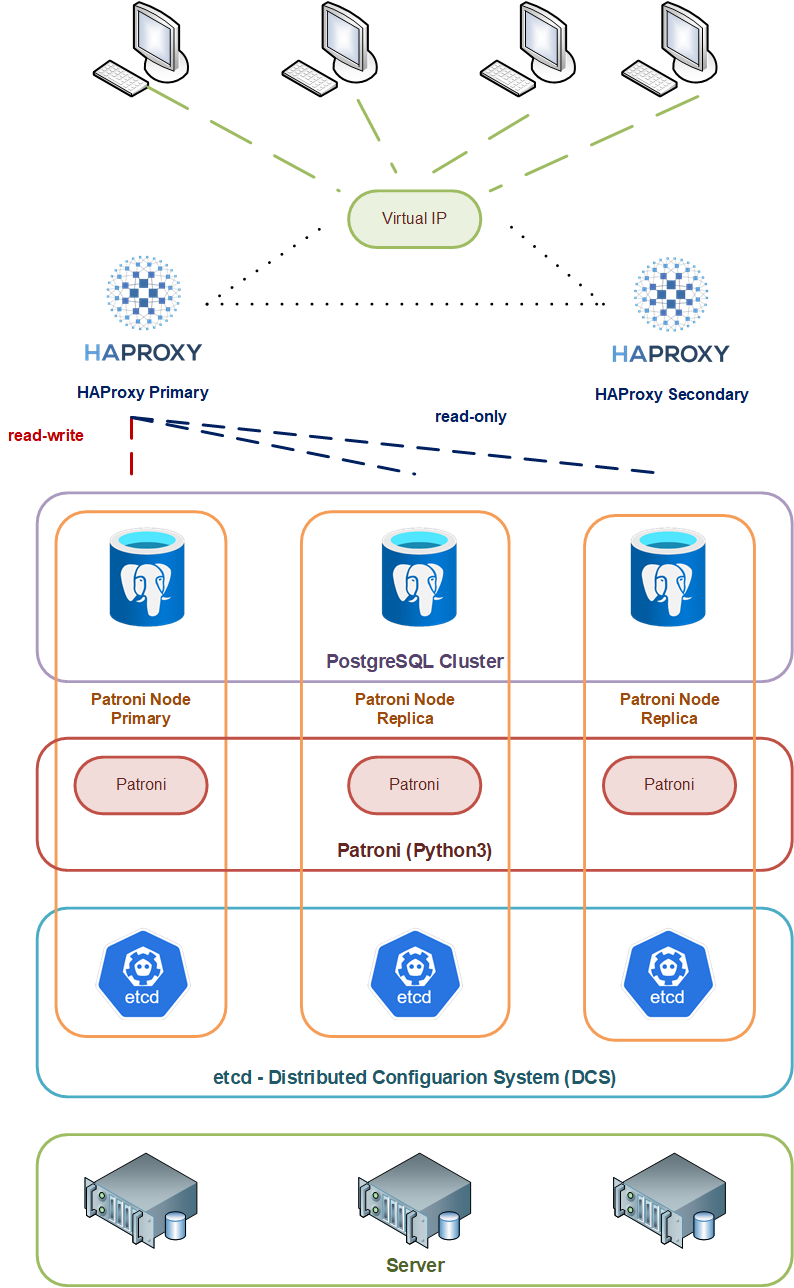
\includegraphics[width=1\linewidth]{source/implementation/evaluation/postgresql_ha_solutions/patroni_architecture}
        \caption{Patroni-Architektur}
        \label{fig:patroni-architecture}
    \end{figure}
\end{flushleft}